\documentclass [12pt ,a4paper,openany]{book}
\special{papersize=210mm,297mm}
\setlength{\topmargin}{0in}
\usepackage[utf8]{inputenc}
\usepackage[italian]{babel}
\usepackage{graphicx,wrapfig,lipsum}
\usepackage{hyperref}
\usepackage[T1]{fontenc}
\usepackage[utf8]{inputenc}
\usepackage{setspace}
\usepackage[paper=a4paper,margin=1in]{geometry}
\usepackage{cite}
\usepackage{subfig}
\usepackage{float}
\usepackage{titlesec}
\renewcommand{\baselinestretch}{1.25}

%PACCHETTI PER LA MATEMATICA
\usepackage{amssymb}
\usepackage{amsthm}
\usepackage{amsmath}

\fboxsep=10mm%padding thickness
\fboxrule=4pt%border thickness

\begin{document}



\title{Reti neurali: dall'algoritmo di back propagation alle reti profonde }
\author{Alessandro Sassi}
\date{Today}

\titlespacing*{\section}
{0pt}{5.5ex plus 1ex minus .2ex}{4.3ex plus .2ex}
\titlespacing*{\subsection}
{0pt}{5.5ex plus 1ex minus .2ex}{4.3ex plus .2ex}






    
    \begin{titlepage}
        
        \noindent
        \begin{minipage}[t]{0.19\textwidth}
            \vspace{-4mm}{
\includegraphics[scale=1.15]{media_tesi/logo_unimib.pdf}}
        \end{minipage}
        \begin{minipage}[t]{0.81\textwidth}
        {
                \setstretch{1.42}
                {\textsc{Università degli Studi di Milano - Bicocca}} \\
                \textbf{Scuola di Scienze} \\
                \textbf{Dipartimento di Informatica, Sistemistica e Comunicazione} \\
                \textbf{Corso di laurea in Informatica} \\
                \par
        }
        \end{minipage}
        
	\vspace{40mm}
        
	\begin{center}
            {\LARGE{
                    \setstretch{1.2}
                    \textbf{Reti neurali: dall'algoritmo di backpropagation alle reti profonde}
                    \par
            }}
        \end{center}
        
        \vspace{48mm}

        \noindent
        {\large \textbf{Relatore:} Prof. Alberto Dennunzio } \\

        \noindent
        {\large \textbf{Co-relatore:} Dott. Luca Manzoni}
        
        \vspace{14mm}

        \begin{flushright}
            {\large \textbf{Relazione della prova finale di:}} \\
            \large{Alessandro Sassi} \\
            \large{Matricola 807001}
        \end{flushright}
        
        \vspace{36mm}
        \begin{center}
            {\large{\bf Anno Accademico 2017-2018}}
        \end{center}

        \restoregeometry
        
    \end{titlepage}
    

   



\tableofcontents
\chapter{Introduzione}
\section*{L'ispirazione biologica}
%\vspace{-2cm}
Il cervello umano è composto da circa 10 miliardi di neuroni. Nella figura riportata in bassa attorno al nucleo di colore verde si estende il corpo cellulare delle cellule neurali , dette \textit{soma} e i canali di input ed output che la circondano la collegano a circa altri 10000 (dieci mila) neuroni.
Ogni neurone riceve degli stimoli elettrochimici dai neuroni circostanti attraverso i proprio dendriti. Se la somma degli input elettrici è potente abbastanza il neurone trasmette a sua volta un segnale elettrochimico lungo l'assone , che viene diffuso a tutti quei neuroni i cui dendriti sono connessi alle terminazione del neurone in oggetto.
Per quel che vedremo in seguito è importante sottolineare come il neurone attivi il segnale in uscita solo se il segnale in ingresso totale raggiunge un certo livello, a quel punto il neurone attiva il proprio impulso, secondo un unico livello di segnale, ovvero, non ci sono sfumature di attivazione, o il segnale in uscita viene propagato o non viene propagato, non esistono segnali di potenza variabile da distribuire verso i neuroni connessi.
Il nostro intero cervello è quindi composto interamente da questa fitta rete di cellule, i neuroni, che comunicano fra loro attraverso segnali elettrochimici. E' sorprendente vedere come la struttura alla base molto semplice, costituita da una cellula che sommando dei segnali in ingresso si attiva , o meno, comunicando con altre cellule attraverso segnali in uscita, riesca nel suo complesso reticolo di interazioni a svolgere funzioni complicate come quelle del cervello nella sua totalità.
Lo studio del cervello e la sua comprensione ha potuto ispirare i modelli scientifici e matematici che oggi danno vita a quelle che sono dette oggi \textit{reti neurali artificiali (ANN)}.

\begin{figure}

\centering

\subfloat[][\emph{An impression of a real neuron. This image is a light microscope photograph by John Anderson, Institute for Neuroinformatics, Zurich, Switzerland.  }]
{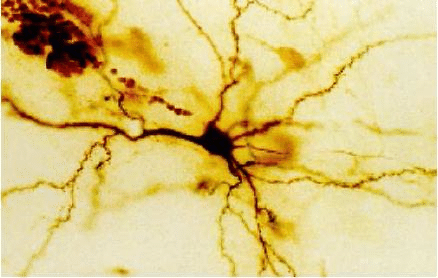
\includegraphics[width=.65\textwidth]{media_tesi/real_neuron.png}} \\
\subfloat[][\emph{A biological neuron model}]
{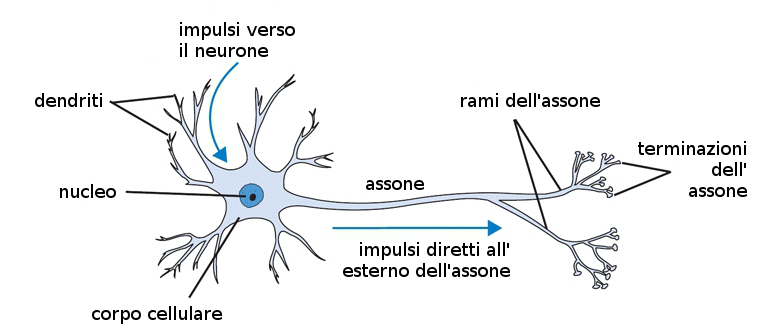
\includegraphics[width=.65\textwidth]{media_tesi/neuron_model.png}} \\

\label{fig:subfig}
\end{figure}

\section*{La storia delle reti neurali}
La capacità dei computer di andare oltre la programmazione verso delle primordiali forme di apprendimento si sviluppò inizialmente come il tentativo di due scienziati di meglio comprendere il funzionamento dei nuroni nel cervello.
Era il 1943 e il neurofisiologo Warrent McCulloch e il matematico Walter Pitts svilupparono con dei circuiti elettrici una semplice rete neurale che modellava i neuroni biologici.
Nel 1949 Donald Hebb scrisse \textit{L'organizzazione del Comportamento} in cui affermava di come i percorsi neurologici tendessero a rinforzarsi e a diventare più solidi mano mano che questi venivano allenati e utilizzati. Un lavoro che troverà conferme in studi successivi e documentati nel saggio di Nicholas Carr del 2010, in cui si fa riferimento alla plasticità del nostro cervello e alla capacità dei nostri neuroni di rinforzare i loro collegamenti man mano che vengono "allenati".
(PENSARE A DOVE METTERE LA CITAZIONE DI CARR CHE TROVO NELLA MAIL A CABITZA)
Nel frattempo i calcolatori diventavano più potenti e sul finire degli anni '50 Bernard Widrow e Marcian Hoff della Stanford University svilupparono "ADALINE" and "MADALINE". La prima era in grado di riconoscere dei pattern binari nel linee telefoniche e predire i successivi bit in ingresso; la seconda fu la prima rete neurale ad essere applicata in un problema del mondo reale, ovvero era in grado , grazie a dei filtri adattivi (COSA SONO000??) di eliminare gli echi nel chiamate al telefono. Questo dispositivo , per quanto datato e primitivo funziona così bene da avere ancora oggi una sua validità commerciale.
Nel corso degli anni , nonostante i primi buoni risultati delle reti neurali l'architettura di von Neumann si impose sulla scena dello sviluppo dei calcolatori, nonostante von Neumann stesso suggerisse di apprezzare l'approccio dell'imitazione delle funzionali neurali.
Inoltre all'epoca furono pubblicati degli articoli scientifici, basati però su un presupposto erroneo, ovvero la non derivabilità delle funzioni di apprendimento (CERCARE DI CAPIRE MEGLIO), che raffreddarono gli entusiasmi per questa tecnologia e con questi gli investimenti per ulteriori sviluppi. Inoltre i primordiali successi condussero ad esagerare potenziale ed aspettative nei confronti delle reti neurali, generando in un primo momento clamore e diffidenza, paura anche rispetto a quallo che avrebbe potuto costituirsi come rapporto uomo-macchina e in seguito in delusione verso le aspettative non ripagate. 
Arrivando agli anni '70: nel 1972 furono sviluppate indipendentemente da Kohonen e Anderson delle reti molto simili che si basavano su una matematica matriciale ; del 1975 è invece la prima rete multistrato non supervisionata.

L'interesse verso le reti neurali artificiali si rinnovò nel 1982 quando  John Hopfield della Caltech (USA) presentò un paper all'Accademia Nazionale delle Scienze. In questo documento presentava l'opportunità di rendere le macchine più utili ed efficienti usando reti bidirezionali rompendo con la tradizionale idea di reti in cui i sengali si propagassero in un'unica direzione. Nello stesso anno altri due ricercatori : Reilly e Cooper usarono reti "ibride" che applicavano differenti strategie di risoluzione per ognuno dei diversi strati della loro rete. Ancora nel 1982 una spinta ai finanziamenti in questo settore arrivò da una conferenza congiunta tra studiosi statunitensi e giapponesi sul tema. Vedendo i nipponici in vantaggio sullo sviluppo di queste tecnologie gli americani decisero di aumentare le risorse a disposizione della ricerca.

Nel 1986 arriviamo ad una svolta che diventa centrale nel corso di questa relazione, ovvero, lo sviluppo dell'idea del backpropagation error. Tre gruppi indipendenti di sviluppatori, tra i quali compariva David Rumelhart, un ex professore di Stanford del dipartimento di psicologia, arrivarono sempre indipendentemente all'idea  di distribuire gli errori prodotti dalla computazione della rete su tutta la rete stessa in modo da riprogrammarne i parametri e farla apprendere dai propri errori.
Quelle che prima abbiamo chiamato reti "ibride" avevano solo due layer mentre queste nuove reti a retropropagazione dell'errore presentavano molti livelli e , dato lo stato dell'arte degli hardware del tempo, erano ritenute molto lente; e così hanno proseguito ad essere, tanto che negli anni 2000, le computazioni potevano richiedere settimane intere. Così è stato finché i recenti sviluppi degli ultimi anni hanno messo a disposizione delle reti hardware performanti e notevoli quantità di dati da cui le reti possano trarre informazioni ed imparare \cite{stanford_history}.

\section*{I diversi tipi rete neurale}
Al giorno d'oggi le reti neurali sono tante e diverse tra loro, vengono riconosciute con l'utilizzo di sigle sempre più lunghe e in questa sezione vedremo alcune delle principali. Ad alcune accenneremo solamente mentre altre non verranno nemmeno citate per via del loro numero elevato.
Le reti neurali biologiche hanno ispirato le reti neurali artificiali che vengono utilizzate per approssimare delle funzioni che non sono conosciute a priori \cite{wiki:tipi} e questo costituisce, semplicisticamente, un ribaltamento del classico paradigma con cui usiamo i computer: la programmazione infatti usa funzioni impostate dal programmatore per computare dei dati in output mentre le reti neurali cercano di creare una funzione a partire da dati forniti.
e questo costituisce, semplicisticamente, un ribaltamento del classico paradigma con cui usiamo i computer: la programmazione infatti usa funzioni impostate dal programmatore per computare dei dati in output mentre le reti neurali cercano di creare una funzione a partire da dati forniti.
Le reti feedforward furono le prime reti ad essere pensate e sono anche le più semplici. Sono costituite da diversi strati (\textit{layers}), che possono essere di input per i dati di apprendimento, nascosti o di output.
Il perceptrone può essere visto come modello di un neurone biologico e può approssimare nella sua semplicità dei circuiti logici. Gli strati delle FF sono tutti collegati fra loro e il flusso dei dati viaggia in una sola direzione, senza mai formare cicli, dallo strato di input, attraverso gli strati nascosti fino allo strato di output. Questa rete viene definita profonda all'aumentare degli \textit{hidden layers} che si nascondono fra input ed output e prendono il nome di \textit{deep feedforward neural networks} (SPECIFICARE SE ESISTE UNA DIFFERENZA SOSTANZIALE, DEL TIPO : UNA VOLTA C'ERANO SOLO QUELLE NON PROFONDE O PERKE HANNO CREATE QUELLE PROFONDE, QUALE ERA L'ESIGENZA CHE LE DISTINGUE).


\begin{figure}[hbtb]
\centering
\subfloat[][\emph{un perceptrone}]
{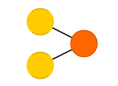
\includegraphics[scale=1.3]{media_tesi/perceptron.png}} \quad
\subfloat[][\emph{una FF}]
{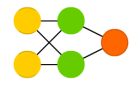
\includegraphics[scale=1.3]{media_tesi/feed_forward.png}} \quad
\subfloat[][\emph{una DFF}]
{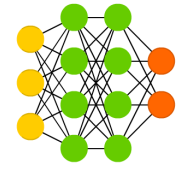
\includegraphics[scale=0.8]{media_tesi/DFF.png}}\\
\caption{Confronto tra tipologie diverse di algoritmi}
\label{fig:subfig}
\end{figure}

Esistono poi anche le \textit{radial basis network} (RBF)che altro non sono che reti feedforward (e che possiamo schematizzare proprio come la FF in figura sopra) ma con una funzione di attivazione radiale di base. Non tutte le reti prendono il nome dalla propria funzione di attivazione ma questa sembrava avere particolari speranze nel 1988, quando uscì il documento che la presentava poiché la funzione che stava alla sua base era in grado di interpolare in spazi di molte dimensioni.(PERCHÈ QUESTA SI ALLORA ????)
 
%------------------------------------------
\begin{wrapfigure}{R}{7.0cm}
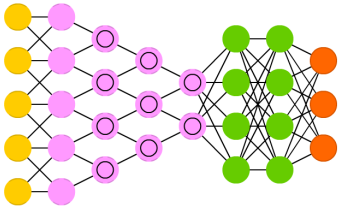
\includegraphics[scale=0.7]{media_tesi/DCN.png}
\caption{Un perceptrone (P).}\label{wrap-fig:1}
%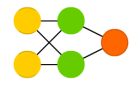
\includegraphics[scale=1.4]{media_tesi/feed_forward.png}
%\caption{rete convoluzionale profonda (DCN).}\label{wrap-fig:1}
\end{wrapfigure} 
%------------------------------------------
Un altro caso speciale o un evoluzione delle FF sono le \textit{reti convoluzionali profonde} (\textit{deep convolutional network , DCN}) il cui utilizzo primario è il processing delle immagini e in alcuni casi anche degli input audio. Si ispirano a quelle che è il funzionamento del sistema visivo degli uomini.
Le reti convoluzionali sono in grado di riconoscere soggetti nelle immagini sapendo quindi fare una classificazione in un insieme di immagini che gli vengono sottoposte. Le DCN scansionano le immagini partendo da piccoli blocchi di pixel vicini tra loro e individuano le caratteristiche delle immagini porzione dell'immagine per porzione, fino a classificare l'immagine nella sua totalità.
Diversamente delle tradizionali FF i layer di mezzo non sono collegati nodo per nodo fra loro, piuttosto i nodi vicini sono collegati ad un intorno dei nodi vicini nello strato successivo. Questo vuole ispirarsi al modo in cui il nostro campo visivo funziona e reagisce agli stimoli esterni. Man mano che il segnale fluisce lungo la rete attraversa strati costituiti da sempre meno nodi fino ad arrivare alla terminazione della rete in cui viene "attaccata" una piccola rete FF che consente di processare ulteriormente i dati e fare nuove astrazioni.

Un recente sviluppo , del 2014, delle reti che sembra essere promettente è la combinazione di due reti insieme. Di solito vengono associate tra loro FF e reti convoluzionali e si impostano in modo tale che esse si contrappongano nello svolgere dei compiti. Immaginiamo un pittore che dipinge su una tela un gatto , in sua compagnia un giudice verifica la qualità del lavoro confrontandolo che un insieme di fotografie di gatti reali; il pittore si allena a ritrarre sempre più fedelmente i gatti e il giudice viene sfidato nel giudicare via via se il gatto sottopostogli dall'amico sia una fedele riproduzione artistica o una foto reale. Ecco nelle reti \textit{GAN}, come sono abbreviate, una delle due fa un lavoro di generazione mentre l'altra fa un lavoro di giudizio, in pratica una genera contenuti che vengono giudicati dall'altra e si allenano vicendevolmente nel giudicare una l'operato dell'altra, spingendo la seconda a produrre contenuti sempre più difficili da predire mentre la prima viene allenata dalla seconda , che producendo via via lavori sempre più approssimabili a quelli dell'insieme di confronto.

Abbiamo parlato fin'ora solamente di reti in cui i segnali partendo da uno strato di input si propagano unidirezionalmente verso la fine della rete. E' giusto annoverare brevemente anche quelle reti che invece formano dei cammini ciclici fra i loro nodi.
\chapter{L'algoritmo di Backpropagation }
\section{L'idea dell'apprendimento}
Cosa significa apprendere? Una domanda non così scontata per un azione che a diversi livelli compiamo per tutta la nostra vita. Ci troviamo ad imparare memorizzando concetti, dati, stimoli sensoriali dai cinque sensi e rielaboriamo il tutto nel nostro cervello producendo idee nuove che derivano dagli elementi di partenza conservati nella nostra memoria.

Un esempio banale è il contatto con un oggetto, da una singola esperienza generalizzeremo l'idea che gli oggetti analoghi a quello con cui abbiamo avuto a che fare procurino le medesime sensazioni. Ma cosa accade se l'esperienza è più complessa? Ad esempio potremmo toccare un ferro da stiro bollente e farci l'idea che quell'oggetto dalla data forma del ferro sia intrinsecamente caldo, ma toccandolo in un momento in cui è spento non ci accadrebbe nulla, anzi percepiremmo il freddo della piastra metallica. La moltitudine di esperienze per contesti affini può fornirci un'idea più chiara del perché di determinati avvenimenti. Avvicinandoci ad un ferro da stiro collegato alla corrente elettrica con la spina avremmo un ulteriore elemento di ragionamento in base al quale fare nuove ipotesi sullo stato dell'oggetto: conoscendo come funzionano gli elettrodomestici potremmo pensare che se il ferro è attaccato alla corrente potrebbe essere acceso e quindi caldo, potremmo pensare che sia rimasto attaccato alla corrente perché nessuno si è preoccupato di staccarlo e che quindi, passato del tempo, sia ormai freddo e possa essere riposto senza bruciarsi. Tutto lineare e chiaro, sono intuizioni semplici per una persona adulta che ha vissuto una simile scena tante volte. 
\\
Come cambiano le cose se proviamo ad immedesimarci in un piccolo bambino? Sarà probabilmente la prima volta che vedremo questo oggetto cuneiforme e non avremo esperienze pregresse per deliberare quale tipo di interazione sia più intelligente avere con esso. Un bambino di un anno infatti non può sapere a cosa serve quell'oggetto, non può sapere che appartiene ad una classe degli oggetti della vita che può trovarsi nel duplice stato di acceso/spento, non può sapere che questi oggetti hanno un filo che li collega al muro e non può sapere che da quel filo passa l'energia necessaria a renderlo funzionante. Le esperienze ci insegnano a comprendere, inferire idee a partire dalla somma di altre. Il bimbo crescendo imparerà a capire che il ferro lo utilizza la mamma in determinate situazioni, imparerà a capire che solo una parte dell'oggetto può bruciare e capirà che dopo diverso tempo che la mamma ha terminato di adoperarlo non brucerà più. Ma questa conoscenza da cosa sarà data? Sarà data con la serie di evidenze avute dal bambino nel toccare il ferro: ci saranno state volte in cui, vispo di curiosità, lo avrà avvicinato per vederlo meglio e sfiorandolo si sarà bruciato; altre volte la mamma, certa della sua esperienza gli avrà mostrato l'oggetto per farglielo conoscere e avvicinandolo non si sarà fatto male. Nella rete intricata di esperienze, sensazioni e fatti tangibili il cervello del bimbo imparerà a dare maggior peso ad alcuni elementi cognitivi piuttosto che ad altri realizzando dentro di lui una consapevolezza che si alimenta ed arricchisce nel tempo. Il bimbo imparerà a capire che lo stato caldo/freddo del ferro dipenderà in larga parte dalla sua posizione nello spazio: vedendolo infatti riposto sullo scaffale dello sgabuzzino saprà che con probabilità non è stato usato di recente e che quindi non deve bruciare; mentre darà poco peso, sempre nel determinare lo stato dell'oggetto, alla sua disposizione nel tempo: poco importerà che sia mattina o sera, poiché non c'è un preciso momento della giornata in cui la mamma stira. Potrebbe averlo toccato una mattina ed essersi scottato così come potrebbe averlo toccato la sera successiva ed essersi scottato nuovamente... allora capirà che il bruciare del ferro non è legato al momento della giornata. 

A seguito di questa discussione informale possiamo approcciarci alla spiegazione di come agisca l'algoritmo di backpropagation, l'algoritmo che aiuta le reti neurali a dare il giusto peso alle caratteristiche degli elementi che le reti analizzano. 
\section{La matematica dietro a backpropagation}
Il nostro algoritmo viene applicato in modo da modificare ad ogni iterazione i parametri della rete, apprendendo via via la loro configurazione migliore per approssimare la funzione che risolve il nostro problema. Nell'apprendimento supervisionato delle reti feed-forward di cui ci occupiamo facciamo apprendere la rete fornendole un paragone con i risultati aspettati del training set. Nel training set sono quindi presenti i vettori di soluzione per ogni problema. Indichiamo con $ y(x)=(y_{1}, y_{2},\, \dots \, , y_{n})^{T} $ il vettore di $n$ dimensioni di output che ci aspetteremmo in uscita dalla  nostra rete; $y(x)$ è la funzione che la nostra rete vogliamo approssimi, la forma di questa funzione non è data e non si conosce a priori, conosciamo soltanto i suoi valori. BP valuta ad ogni iterazione quanto lontano dal valore atteso è il risultato della rete, computa quindi una funzione dei costi
\begin{equation}
	C(w,b)\equiv\frac{1}{2n}\sum_{x} \parallel y(x)-\hat{y}(x)\parallel^{2}
\end{equation} 


che chiamiamo \textit{errore quadratico medio (MSE)}; $\hat{y}(x)$ invece è a sua volta una funzione dei pesi $w$ e dei bias $b$ e rappresenta il vettore output della rete: in questo modo abbiamo quindi una funzione che mette in relazione il risultato atteso con quello effettivo e che diventa tanto più piccola nel suo valore quanto più $\hat{y}(x)$ approssima $y(x)$. Quindi, se l'intento della rete è produrre un output che approssimi al meglio le soluzione del set di apprendimento, e $C$ ne è la misura, dobbiamo cercare di capire per quali valori questa funzione si minimizza, ovvero trovare per quali valori delle sue $w$ e $b$ variabili l'errore è minimo. 
\\
Per far questo abbiamo bisogno di un metodo. Potremmo pensare di trattare questa minimizzazione con un approccio analitico ma considerando che le variabili in gioco nelle reti reali possono essere anche miliardi questo non è fattibile. 
Facciamo allora ricorso ad un algoritmo, che in diversi passi successivi ci aiuta a trovare il punto di minimo che cerchiamo. Questo algoritmo è il \textit{metodo della discesa del gradiente}, spieghiamo in primis cosa è il gradiente e poi come funziona l'algoritmo.
Data una funzione di due o più variabili, il suo gradiente in un punto $x=(x_{1}, x_{2},\, \cdots \, , x_{n})$ del dominio è il vettore delle sue derivate parziali rispetto a tutte le variabili: $\nabla C \equiv (\frac{\partial C}{\partial x_{1}}, \frac{\partial C}{\partial x_{2}}, \cdots, \frac{\partial C}{\partial x_{n}})^{T}$. Questa è solo una formula matematica e non ci da bene idea di cosa stiamo parlando. Dobbiamo allora rifarci ad uno scenario reale per capire meglio cosa sia il gradiente; la realtà è fatta di tre dimensioni quindi rimaniamo in uno spazio tale per spiegarci meglio: se fossimo in una valle e avessimo una palla perfettamente tonda, il gradiente è il vettore della direzione lungo la quale la funzione cresce maggiormente e, di contrario, $-\nabla C$ è la direzione in cui la palla si muoverebbe se, appoggiata a terra, venisse lasciata libera di rotolare lungo il pendio della valle. In una tale ipotesi le variabili libere non sono $n$ come abbiamo generalizzato, ma sono soltanto due $v_{1}, v_{2}$ (usiamo le $v$ e non le $x$ per separare la spiegazione dalla sua metafora). Possiamo vederne una rappresentazione di quanto detto nella figura \ref{gradiente}.

\begin{figure}[hbtb]
\centering
{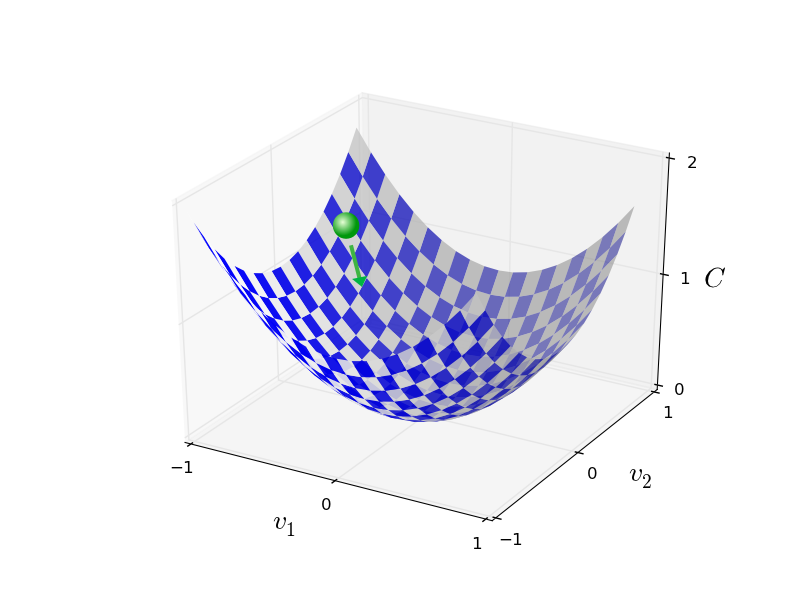
\includegraphics[width=.55\textwidth]{media_tesi/valley_with_ball.png}}
\caption{Il grafico della funzione $C(v_{1}, v_{2})$ con la pallina verde che rappresenta il punto in analisi e l'opposto del vettore gradiente spiccato in esso, ad indicare in quale direzione muoverebbe nella discesa}
\label{gradiente}
\end{figure}

Se ora abbiamo un'idea più chiara di cosa sia il vettore gradiente spieghiamo in cosa consiste il metodo della discesa che lo utilizza. Ipotizzando la stessa metafora della valle vogliamo sfruttare il fatto che la discesa della pallina si arresterà nella parte più bassa dalla depressione. Il nostro metodo computa una discesa simile ma diversa nel fatto che il percorso che farà la nostra pallina non approssimerà la discesa \textit{fisica} che avverrebbe nella realtà. Per cui il nostro metodo non si rifà alle equazioni della dinamica di Newton, è un pò diverso. Per ora sappiamo che, dato un punto sulla superficie di una valle, la direzione opposta a quella del gradiente è quella in cui la palla si muoverebbe se fosse libera di scendere; nel nostro metodo seguiamo un percorso di discesa fatto di tanti piccoli passi che prevedono, partendo da un punto, di muoversi verso $-\nabla C$ per un piccolo tratto. Mossi nel nuovo punto, che chiamiamo $P_{2}$, ricalcoleremmo il gradiente $\nabla C(P_{2})$ e faremmo un altro piccolo passo in direzione $- \nabla C(P_{2})$. Si capisce che questo metodo va iterato a lungo per scendere lungo la valle fino ad arrivare nel suo punto più basso. Tra un iterazione $k$ e la successiva $k+1$, ci saremo spostati dal punto $P_{k}$ al punto $P_{k+1}$ per cui $ \Delta P= P_{k+1}-P_{k}=-\eta \nabla C$ dove $\eta$ è un piccolo parametro positivo detto il \textit{learning rate} che fornisce un indicazione di quanto grande sia la distanza percorsa fra un iterazione e l'altra nell'algoritmo; va da se che se il $\eta$ cresce l'algoritmo procede più speditamente, ma questo potrebbe portare anche a degli errori. Ritorniamo dal parallelo con la valle, la palla e le variabili $v$ alla nostra funzione dei costi $C(w, b)$ e vediamo come il metodo del gradiente funzioni con più di due variabili, anche se di questa situazione non potremo avere una visualizzazione. Cosi come ci spostiamo da un punto all'altro nella valle, aggiornando le due variabili della nostra posizione, ora aggiorniamo le variabili della funzione dei costi, ovvero $w$ i pesi e $b$ i bias. Le regola per aggiornare queste componenti sarà:
\begin{equation}
w_{k}\rightarrow w'_{k}=w_{k}-\eta \dfrac{\partial C}{\partial w_{k}}
\end{equation}
\begin{equation}
b_{l}\rightarrow b'_{l}=b_{l}-\eta \dfrac{\partial C}{\partial b_{l}}
\end{equation}
dove $k$ e $l$ variano, rispettivamente, tra tutti i pesi e i bias della rete. Ripetendo questa regola arriveremo a trovare il minimo della funzione.
%\begin{center}
%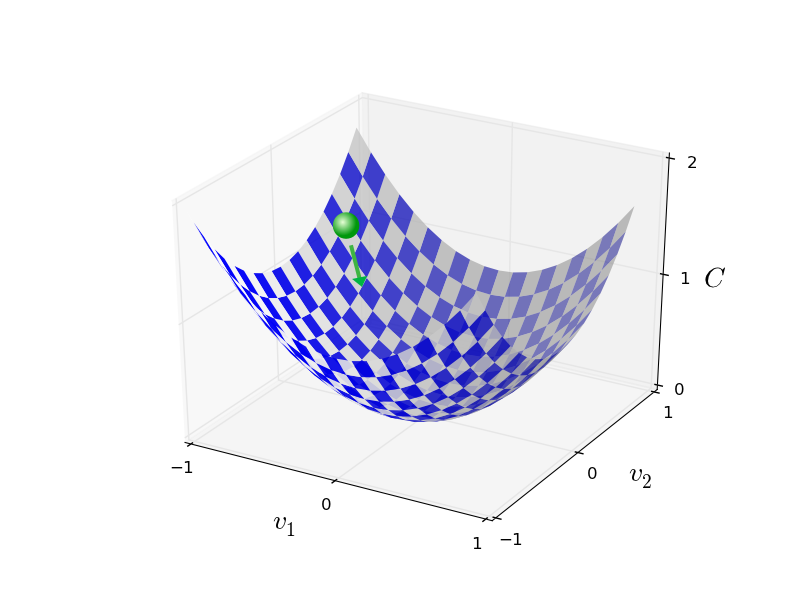
\includegraphics[width=0.5\textwidth]{media_tesi/valley_with_ball.png}
%\caption{Il grafico della funzione $C(v_{1}, v_{2})$ con la pallina verde che rappresenta il punto in analisi e il vettore gradiente spiccato da esso, ad indicare in quale direzione moverebbe nella discesa}
%\end{center}
\\
Ora che abbiamo spiegato come funziona il gradiente dobbiamo andare più a fondo a spiegare come interagiscono fra loro i neuroni collegati, come si attivano e come propagano il proprio segnale.
Ogni neurone $j^{th}$ è collegato (stiamo sempre parlando del caso delle reti feed forward) ai neuroni dello strato precedente dall'arco di peso $w^{l}_{jk}$ (cioè dal neurone $k$ in $l-1$ al neurone $j$ in $l$) e la sua attivazione viene determinata da una computazione fatta sui segnali in ingresso, più precisamente è la somma delle attivazioni dei neuroni dello stato precedente a lui collegati, moltiplicati per il peso del loro arco verso $j^{th}$ più una quantità $b_{j}$ specifica del neurone $j$ nello strato $l$, questa somma prende il nome di $z^{l}_{j}$. 

\begin{equation}
\displaystyle a^{l}_{j}=\sigma\left( z^{l}_{j}\right) = \sigma \left( \sum_{k}w^{l}_{jk}a^{l-1}_k +b^{l}_{j} \right)
\end{equation}

Spieghiamo brevemente cosa è $\sigma$. Ogni neurone riceve input dagli strati precedenti e internamente deve decidere se propagare a sua volta lo stimolo o meno. In biologia abbiamo già anticipato che i neuroni, una volta eccitati, non hanno una via di mezzo nel rispondere al segnale, per cui, o propagano a loro volta lo stimolo nella rete ``accendendosi''  oppure rimangono in quiete senza reagire. Nelle reti neurali la funzione di attivazione di solito non emette un segnale binario, piuttosto propaga vari livelli d'intensità del segnale. $\sigma$ rappresenta quella classe di funzioni sigmoidali che ben si adattano a rappresentare l'attivazione dei neuroni e che hanno lo scopo di normalizzare gli output nel range da $0$ a $1$. Quindi, se un neurone reale può veder rappresentata la propria funzione di attivazione come una funzione a gradino una sigmoide è la versione addolcita della funzione gradino, come mostriamo qui sotto con il plot della funzione sigmoide:
\begin{equation}
	\sigma(z)=\dfrac{1}{1+e^{-z}}
\end{equation}

%\begin{figure}[hbtb]
%\centering
%{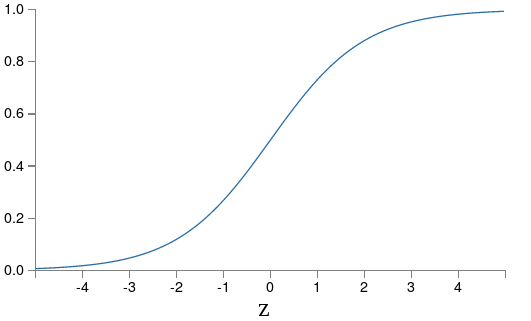
\includegraphics[width=.45\textwidth]{media_tesi/sigmoide.png}}
%\caption{Il grafico della funzione sigmoide $\sigma(z)$}
%\label{fig:subfig}
%\end{figure}

\begin{figure}[hbtb]
\centering
\subfloat[][\emph{Grafico della funzione sigmoide $\sigma(z)$}]
{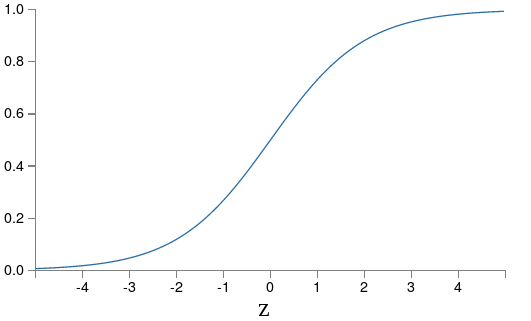
\includegraphics[width=.45\textwidth]{media_tesi/sigmoide.png}} \qquad
\subfloat[][\emph{Grafico ReLu}]
{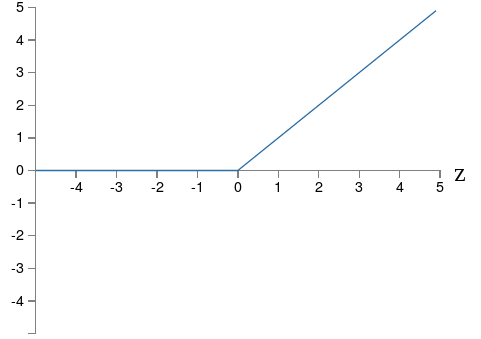
\includegraphics[width=.41\textwidth]{media_tesi/relu.png}} \\
\caption{Confronto tra due funzioni di attivazione}
\label{fig:subfig}
\end{figure}

La sigmoide non è l'unica funzione adatta per le reti neurali. Si usa anche $tanh$ oppure, un altra funzione è la \textit{ReLu}(Rectified Linear Unit)  $\displaystyle f(z)=max(0,z)$ che venne resa popolare quando la \textit{AlexNet} vinse la sfida \textit{ImageNet}nel 2012, un concorso che premia i migliori algoritmi per l'\textit{object detection} e la classificazione delle immagini. La \textit{AlexNet} usava \textit{ReLu} come funzione di attivazione e da quel momento in poi altri la adottarono ai propri scopi rendendosi conto, in via empirica, che funzionava meglio di quanto usato fino a quel momento \cite{krizhevsky2012imagenet}. Non è perfettamente chiaro cosa la renda migliore ma si pensa che la convergenza del metodo del gradiente venga velocizzata da \textit{ReLu} grazie alla sua semplicità e alla sua capacità di non saturarsi\cite{cs23}.

L'output di un neurone è denotato da $ a^{l}_{j} $ per ogni neurone $j$ nello strato $l$, possiamo definire un vettore contenente questi output per tutti gli $n$ neuroni di quello strato $a^{l} = \left[a^{l}_{1},a^{l}_{2}, \cdots, a^{l}_{j}, \cdots, a^{l}_{n}  \right] $. Vediamo ora come di strato in strato i neuroni si attivano fra loro e per questo adottiamo una notazione matriciale di quanto abbiamo appena visto: denotiamo allora una matrice $w^{l}$ dei pesi per ogni layer della rete, dove le sue entry sono $w^{l}_{kj}$ i vari pesi che legano i neuroni fra lo strato $l-1$ ed $l$ e denotiamo, allo stesso modo di $a^{l}$ anche il vettore dei \textit{bias} $b^{l}$ per il livello $l$ e riscriviamo la formula 3 come:
\begin{equation}
	a^{l}=\sigma\left( w^{l}a^{l-1}+b^{l}\right)
\end{equation}
\\
La propagazione del calcolo degli output dei singoli livelli procede verso il livello finale, l'\textit{output layer}, e una volta calcolato l'errore nella funzione dei costi, $C$, questo errore viene propagato in senso opposto fino al layer degli input. Spieghiamo meglio quale è il senso di questo ``propagarsi''. 
$C(w,b)$ è stata definita in (1) e viene calcolata sull'output layer $a$ della rete, questo che possiamo indicare per chiarezza come $a^{out}$ per esplicitare a quale livello sia riferito è calcolato a sua volta come indicato nella (5) ed   è quindi funzione dei pesi e dei bias del livello che lo precedono: $ a^{out}(w^{l},b^{l}, a^{l})$ dove $l$ è l'ultimo \textit{hidden layer}, quello prima di \textit{out}; ma compare anche $a^{l}$, questo in catena è una funzione di pesi, attivazioni e bias di $l-1$. Vediamo quindi come in verità tutta la funzione dei costi non sia altro che una lunghissima e imponente funzione composta, che richiama i parametri dei livelli sottostanti. Compreso questo possiamo dire che se la $C$ è una funzione composta dei pesi e dei bias di tutti i suoi sottolivelli e quindi della rete in generale; possiamo cercare di capire in che modo questi parametri, lungo la rete, contribuiscano alla definizione di $C$ e in ultima analisi di come contribuiscano alla quantità dell'errore espresso da $C$ e della rete nel suo complesso; in questo senso l'errore viene retropropagato lungo la rete. Per vedere che peso ha complessivamente un peso $w_{k}^{l}$ si calcola la sua derivata parziale $\frac{\partial C}{\partial w_{k}^{l}}$ ma per poter far questo bisogna procedere livello per livello. Abbiamo detto che $C$ è una funzione composta ed è necessario partire livello di output e andare indietro per calcolare le derivate dei pesi più in profondità applicando la \textit{chain rule} delle funzioni composte $(f \circ g)'=(f' \circ g) \cdot g' $.
\begin{equation}
	C(a^{out})= C( a^{out}(w^{l},b^{l}, a^{l})) = C( a^{out}(w^{l},b^{l}, a^{l}(w^{l-1},b^{l-1}, a^{l-1}))) = \cdots
\end{equation}
La formula sopra dovrebbe rendere l'idea di come si procede a comporre la funzione costi, innestando via via i pesi e i bias. Per trovare la derivata $\frac{\partial C}{\partial w_{k}^{m}} $ di un peso di un neurone nel livello $m$ dovremo quindi calcolare prima di lui tutte le derivate delle funzioni che lo contengono:
\begin{equation}
	\dfrac{\partial C}{\partial w_{k}^{m}} = \dfrac{\partial C}{\partial a^{out}}\cdot \dfrac{\partial a^{out}}{\partial a^{l-1}} \cdot \dfrac{\partial a^{l-1}}{\partial a^{l-2}}\cdot \; \cdots \; \cdot \dfrac{\partial a^{m}}{\partial w^{m}_{k}}
\end{equation} 
In questo senso la procedura avanza verso la base della rete, calcolando tutte le derivate parziali rispetto ai $w$ e ai $b$ della rete (per ogni neurone di ogni layer); il che corrisponde ad avere calcolato il gradiente della funzione dei costi:
\begin{equation}
	\nabla C = \left[ \dfrac{\partial C}{\partial w_{1}^{1}}, \dfrac{\partial C}{\partial w_{2}^{1}}, \cdots, \dfrac{\partial C}{\partial w_{n}^{1}},\dfrac{\partial C}{\partial b_{1}^{2}}, \cdots \dfrac{\partial C}{\partial b_{2}^{2}}, \cdots \right] 
\end{equation} 
Una volta ottenuto il gradiente di $C$ possiamo procedere all'aggiornamento dei pesi, l'apprendimento della rete si basa infatti su questo, sulla modifica dei suoi parametri interni in modo che dal loro cambiamento scaturisca un comportamento complessivamente diverso (migliore) nei confronti degli input che le vengono passati e con diversi training riesca a darci i risultati che speriamo.
La regola di aggiornamento di un generico peso è questa:
\begin{equation}
	w_{j}^{l +} = w_{j}^{l} + \eta \dfrac{\partial C}{\partial w_{j}^{l}}
\end{equation}
che altro non è che la procedura della discesa del gradiente spiegata in precedenza.

\section{I miglioramenti}
\subsection*{Migliorare backpropagation attraverso diversi approcci sulla discesa del gradiente}

L'algoritmo di backpropagation si basa sull'ottimizzazione di una funzione d'errore tra l'output della rete e il risultato desiderato. La funzione in questione ha come variabili i pesi associati ai collegamenti tra i vari neuroni della rete e i loro bias. Nella sua versione più semplice la funzione cerca il proprio minimo seguendo la direzione del proprio gradiente.
Venendo alle variazioni su questo metodo; furono proposti il \textit{metodo dei minimi quadrati} (in inglese OLS: Ordinary Least Squares) e il \textit{metodo detto di quasi-newton} (che è una variazione sul canonico metodo di Newton) che risultano essere però troppo lenti da computare, in special modo nelle reti molto ampie e ad entrare nello specifico il problema per i metodi di quasi-newton è che lo spazio in memoria richiesto per salvare una approssimazione dell'inversa dell'Hessiana cresce quadraticamente rispetto al numero dei pesi su cui viene effettuato il calcolo \cite{saito1997partial}. Altre tecniche come \textit{BFGS} o il \textit{gradiente coniugato} possono essere in alcuni casi delle valide alternative.
Più genericamente il problema del migliorare l'ottimizzazione dell'errore trova soluzione quando si migliora la capacità di computare la più utile lunghezza di passo possibile (step-lenght) ovvero quanto distante una iterazione deve essere da quella che la precede avendo seguito la direzione del gradiente.
Esistono per questo algoritmi del secondo ordine e del primo ordine, che possiamo vedere a confronto nelle due immagini in Figura \ref{discese}.

\vspace{5 mm}

\begin{figure}[hbtb]
\centering
\subfloat[][\emph{Traiettorie algoritmi del primo ordine}]
{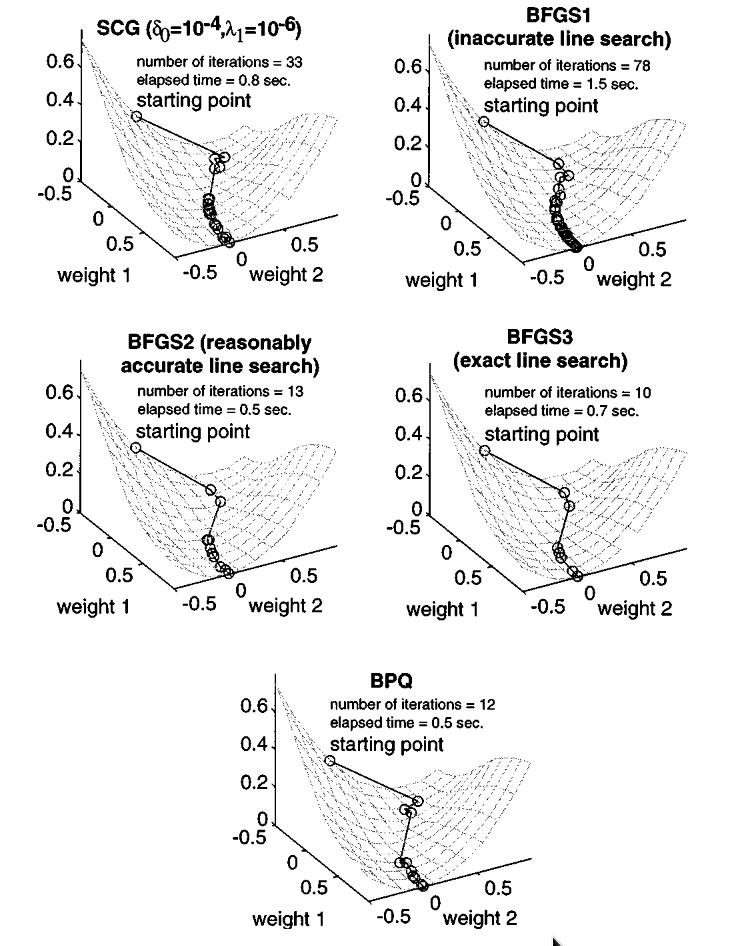
\includegraphics[width=.45\textwidth]{media_tesi/learning_trajectories_of_second_order.jpeg}} \quad
\subfloat[][\emph{Traiettorie algoritmi del secondo ordine}]
{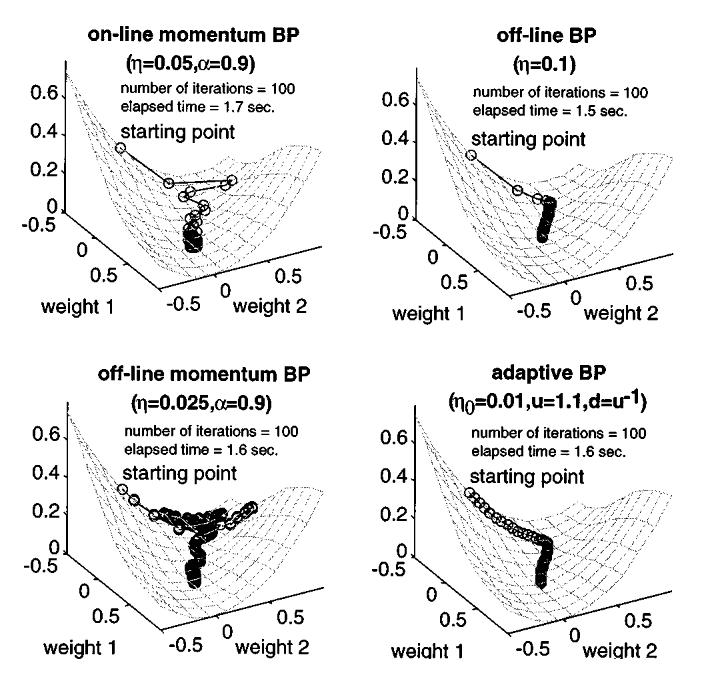
\includegraphics[width=.45\textwidth]{media_tesi/learning_trajectories_of_first_order.jpeg}} \\
\caption{Confronto tra tipologie diverse di algoritmi}
\label{discese}
\end{figure}
\vspace{5 mm}

Si può vedere come l'andamento della traiettoria conduca al minimo in numero inferiori di passi utilizzando algoritmi del secondo ordine.

Per velocizzare BP è stato anche introdotto il momento, che ha lo scopo di ridurre le oscillazioni della traiettoria dovute ad una non proficua scelta della lunghezza del passo per le iterazioni e fu proprio nel 1988 che Robert A. Jacobs, propose quattro euristiche per il miglioramento del tasso di convergenza del backpropagation \cite{nielsen_book}.

Nel 1988 la ricerca aveva già riconosciuto la bontà della procedura BP e si investigavano quegli algoritmi di ricerca dell'ottimo per la funzione di minimo che computassero la discesa del gradiente soltanto localmente (ovvero rimanendo in intorni molto vicini al punto di iterazione). Questo cosidetto \textit{locality constraint} veniva motivato dal fatto che costituiva una buona metafora tecnologica della controparte biologica, le reti neurali, a cui si ispirava e in secondo luogo dall'ipotesi che questi algoritmi \textit{locali} fossero più adatti ad essere processati in parallelo.
Fra le quattro euristiche di Jacobs vi era l'adattamento dei tassi d'apprendimento nel tempo e si spiega che ogni peso della rete dovrebbe avere il proprio tasso d'apprendimento specifico. Le implementazioni di queste euristiche venivano individuate nel \textit{momento} e nella regola d'apprendimento \textit{delta-bar-delta}.
\subsection*{Low complexity NNs}
Alcuni altri indirizzi di miglioramento dell'efficacia delle reti sfruttano il BP per modellare delle reti meno complesse (\textit{low complexity}) che possano essere utili a scopi meno sofisticati. Ad esempio, nelle reti convuluzionali, dove il processo di riconoscimento degli oggetti ha luogo, gli algoritmi vengono eseguiti su GPU che dissipano grandi quantità di energia e un tale scenario non è adatto a scopi dove il livello di dettaglio nel riconoscere gli oggetti non è così elevato. Applicazioni più popolari e frequenti come il riconoscimento facciale nei dispositivi mobili deve per forza di cose girare in locale sui processori embedded che animano gli smartphone, per questo i ricercatori sfruttano varianti del BP per creare reti convuluzionali a bassa complessità. Queste modellano problemi che richiedono meno risorse e possono quindi essere eseguite più velocemente anche sui dispositivi meno prestanti\cite{TSD}.
\subsection*{Le performance con CPU e GPU}
Nella sezione riguardante la matematica di backpropagation abbiamo citato come i calcoli per le attivazioni dei neuroni non vengano eseguiti uno alla volta ma, livello per livello, vengano raggruppati in vettori e matrici non solo per snellire la notazione usata ma anche perché a tutti gli effetti è quello che accade realmente. La quantità di dati coinvolta in una rete neurale può essere davvero notevole, con lo strato di input che può avere fino a migliaia di nodi, per questo le matrici che vengono coinvolte nei calcoli possono diventare molto grandi ed occupare notevoli quantità di spazio in memoria.\\ 

Tale utilizzo di memoria costituisce un limite difficile per la computazione da parte delle CPU, anche quelle multi-core. Le CPU ottimizzano la velocità di calcolo sui singoli processi seriali e sono un'alternativa ad un altro tipo di architettura per processori: le GPU. A detta di Nvidia le GPU furono inventate nel 1999, ma le loro origini risalgono a molti anni prima e datare un nascita per questa tecnologia è quasi impossibile visto che deriva dall'evoluzione di soluzioni tecnologiche affini per scopi che si sono succedute nel corso degli anni. Nel 2007 gli sviluppatori poterono sfruttare le potenzialità di calcolo parallelo anche per applicazioni più generiche grazie alla piattaforma di programmazione \textit{CUDA}. Nel 2009 un documento accademico di Stanford illustrava quanto più velocemente si potesse addestrare delle reti neurali utilizzando metodi con GPU, fino a 70 volte più veloci della controparte con CPU \cite{raina2009large}. Tale approccio consentì l'uso di dataset più ricchi e un aumento dei parametri a disposizione per settare la rete. 

Ma perchè le GPU? Tanta più memoria si necessita per sviluppare i calcoli di queste matrici tanto più l'utilizzo delle GPU migliora le prestazione perché consiste di numerose unità di calcolo semplici che possono agire in parallelo.
\\
Un esperimento presentato da alcuni studiosi nel 2016 comparava due reti neurali nello svolgere il medesimo compito, una implementata su GPU l'altra su CPU. L'esperimento consiste nel riconoscere cifre numeriche scritte a mano, presentate in un dataset chiamato \textit{MNIST}, come quelle in Figura \ref{MNIST}. Presentiamo i risultati delle velocità di computazione nella tabella e nel grafico riportato sotto, dai quali possiamo evidenziare come aver allenato la rete neurale attraverso la GPU aumenti di un fattore molto grande le performance rispetto alla controparte in CPU e che la GPU sia da preferire quando nella rete sono presenti un grande numero di attributi, altrimenti il costo dell'inizializzazione della scheda non verrebbe giustificato dall'incremento delle velocità \cite{brito2016gpu}.

\vspace{15mm}

\begin{figure}[h]
\centering
{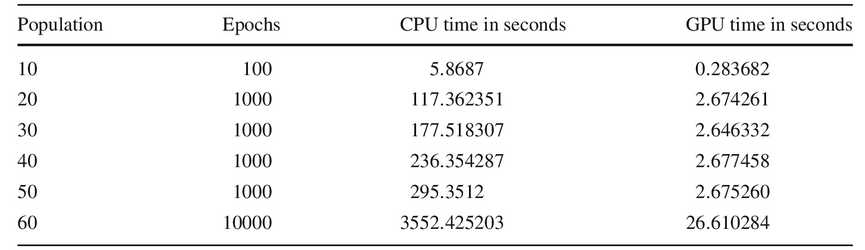
\includegraphics[scale=0.65]{media_tesi/table_experiment.png}}
\caption{Riassunto dei risultati dell'esperimento \cite{brito2016gpu}}
\label{fig:subfig}
\end{figure}

\begin{figure}[h]
\centering
{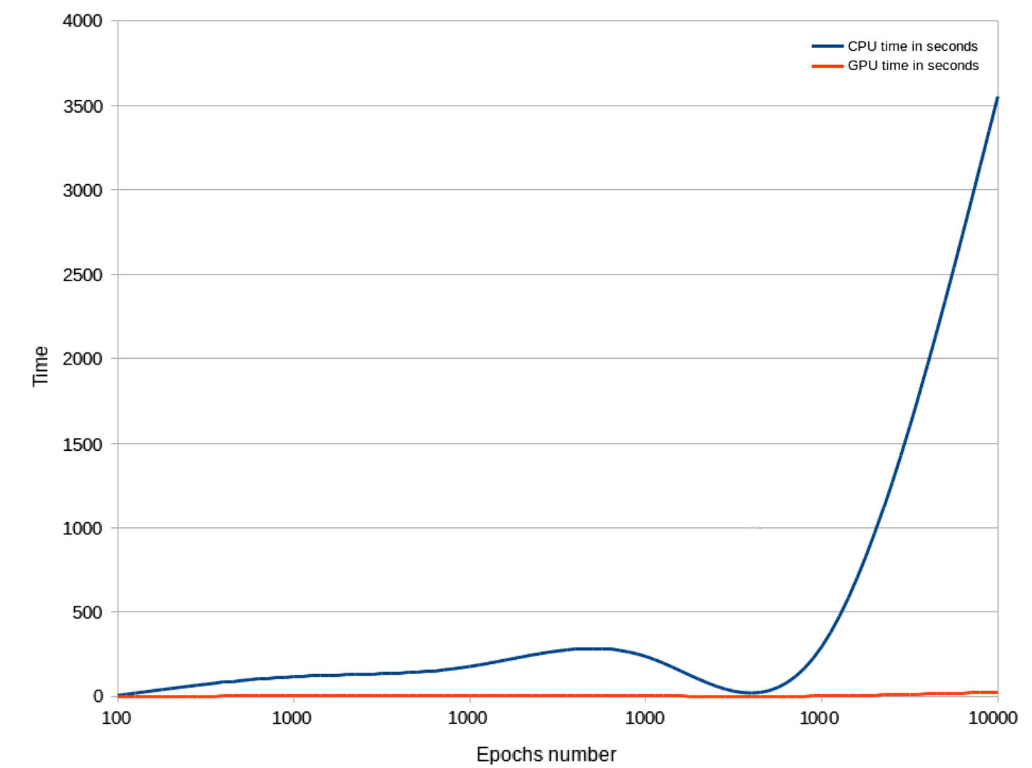
\includegraphics[scale=0.5]{media_tesi/graph_GPU_vs_CPU.png}}
\caption{Il grafico che mostra le differenze tra le velocità di esecuzione tra CPU e GPU \cite{brito2016gpu}}
\label{fig:subfig}
\end{figure}

\begin{figure}[b]
\centering
{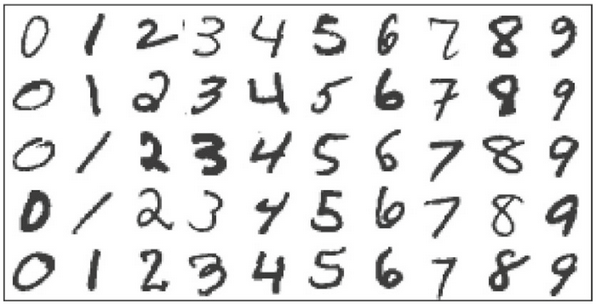
\includegraphics[scale=0.5]{media_tesi/MNIST.png}}
\caption{Un esempio di cifre da riconoscere da parte della reti nell'esperimento}
\label{MNIST}
\end{figure}

%\begin{figure}[hbtb]
%\centering
%\subfloat[][\emph{Traiettorie algoritmi del primo ordine}]
%{\includegraphics[width=.45\textwidth]{media_tesi/}} \quad
%\subfloat[][\emph{Traiettorie algoritmi del secondo ordine}]
%{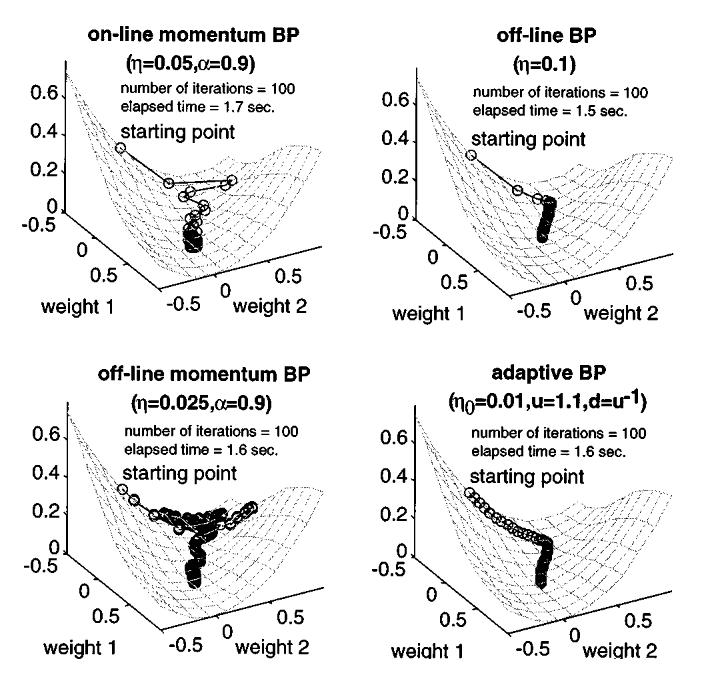
\includegraphics[width=.45\textwidth]{media_tesi/learning_trajectories_of_first_order.jpeg}} \\
%\caption{Confronto tra tipologie diverse di algoritmi}
%\label{fig:subfig}
%\end{figure}

\chapter{I framework per le reti neurali}
\section{Una panoramica}
In questo ultimo capitolo passiamo in rassegna i framework esistenti per l'implementazione di reti neurali. Grazie a loro  lo sviluppo di modelli e il processo di acquisizione dati per l'allenamento dei dati diventa molto più facile e accessibile rispetto ad un tempo. 
\begin{figure}[hbtb]
\centering
\subfloat[][\emph{Keras}]
{
\includegraphics[scale=0.5]{media_tesi/keras_logo.png}} \hspace{1.5cm}
\subfloat[][\emph{Tensorflow}]
{
\includegraphics[scale=0.5]{media_tesi/ts_logo.png}} \hspace{1.5cm}
\subfloat[][\emph{PyTorch}]
{
\includegraphics[scale=0.6]{media_tesi/pytorch_logo.png}} \hspace{1.5cm}
\subfloat[][\emph{Caffe 2}]
{
\includegraphics[scale=0.6]{media_tesi/caffe2_logo.png}} \hspace{1.5cm}
\subfloat[][\emph{theano}]
{
\includegraphics[scale=0.3]{media_tesi/theano_logo.png}} \hspace{1.5cm}
\subfloat[][\emph{mxnet}]
{
\includegraphics[scale=0.4]{media_tesi/mx_logo.png}}\\ 


\caption{I loghi dei principali framework per le reti neurali}
\label{fig:subfig}
\end{figure}

\section{Tensorflow}
Tensorflow  fu creato dal team Brain Google come successore di un precedente sistema per il machine learning conosciuto come \textit{DistBelief} con l'intento di ristrutturare il codice rendendola una libreria più robusta \cite{wiki:tf}. Venne distribuita come progetto open-source nel 2015 e si presenta come un framework di basso livello \cite{oreilly:pytorch_intro} per linguaggi come Python, Javascript, Swift e Java per Android  e le librerie a cui fa a sua volta ricorso per l'implementazione delle parti più critiche sono scritte in C++. \textit{TF} offre compatibilità con le API d'alto livello di \textit{Keras}; esse consentono grazie alla loro modularità e facilità di utilizzo di eseguire velocemente la prototipizzazione di modelli e la sperimentazione delle reti neurali su piattaforme diverse e renderle velocemente funzionanti per il testing \cite{keras}.

Tensorflow rappresenta le computazioni come dei grafi i quali sono composti da due tipi di oggetti: le operazioni, ovvero i nodi del grafo e i tensori, dal cui utilizzo prende il nome, che sarebbero gli archi del grafo.
I tensori sono matrici multidimensionali su cui vengono fatti i calcoli e che contengono i parametri della rete.

Tensorflow gira sia su CPU che GPU, grazie alle librerie di programmazione per schede grafiche \textit{CUDA} e \textit{OpenCL}. Per la sua applicazione specifica è stato progettato da Google un processore dedicato chiamato \emph{Tensor Processing Unit} \textit{TPU}. L'interesse verso un processore dedicato non tanto all'allenamento della rete quanto al suo utlizzo rappresenta un vantaggio per l'applicazione dell'intelligenza artificiale in quegli ambiti dove si predilige una velocità di esecuzione; un esempio può essere un chip dedicato in un dispositivo cellulare, che rende più efficiente determinati task, come il riconoscimento vocale o facciale per quelle applicazioni che ne fanno uso. Google stessa dichiarò che il suo utilizzo nei datacenter aveva ottimizzato le performance di un ordine di grandezza, riducendo il dispendio energetico derivato dal loro utilizzo \cite{gao2014machine}. 

Ts presenta anche diverse problematiche come la sua difficoltà di utilizzo (ecco perchè Keras si appoggia al disopra di TS, come dicevamo in precedenza) e la sua incapacità di scalare linearmente, oltre alle problematiche di distribuire il carico di lavoro su molteplici GPU\cite{quora:mxnet}.

\section{PyTorch}
Questo framework uscì nel 2016 e si ispirò fortemente ad altri framework come \textit{Chainer} e \textit{Torch}. Pytorch si indirizzava le problematiche di adozione che colpivano Torch e a questo proposito si decise di utilizzare come linguaggio d'utilizzo per gli utenti Python. Il suo approccio è un pò diverso da quello di Tensorflow in quanto l'esecuzione delle operazioni nel grafico computazionale avvengono immediatamente mentre in TF il grafico è compilato ed eseguito in un colpo solo e questo rende possibile un debugging più dinamico. Infatti costituisce un rallentamento l'immaginare un modello e dover fare i conti con gli errori della sua progettazione soltanto a termine di questa, è molto più produttivo correggere gli errori via via che si presentano. 

Pytorch è sviluppato e mantenuto dal team per l'intelligenza artificial di Facebook (\textit{FAIR}) e la sua adozione presso gli utenti è stata molto più ampia rispetto a quella del suo predecessore. Viene apprezzato per la familiarità che ricercatori e data scientist avevano già nei confronti di Python mentre a livello commerciale gli vengono preferite alternative in quanto i modelli di PyTorch non sono facilmente portabili su mobile \cite{oreilly:pytorch_intro}.

Negli stessi laboratori di Facebook la strategia è quella di utilizzare PyTorch nella ricerca e Caffe2 per la produzione.

PyTorch offre supporto ai dispositivi CUDA con Python e un frontend C++ \cite{pytorch:docs}. [CHIEDERE COSA SIGNIFICA PERKE NON HO CAPITO MOLTO]

\section{Caffe2}
Arriviamo a quest'altro progetto per le reti neurali sviluppato da Facebook, il più giovane fra quelli che presentiamo. \textit{Caffe2} trae origine da \textit{Caffe}, il quale offriva un ottimo supporto alla produzione di applicazioni che lavorassero bene su larga scala, grazie al suo codice sorgente scritto in C++ \cite{caffe_intro}. Rispetto al predecessore si evidenzia la modularità e il forte orientamento al mondo mobile, con applicazioni nella visione artificiale e il riconoscimento del linguaggio \cite{wiki:caffe2}. Facebook annunciò la pubblicazione open-source di Caffe2 il 18 aprile 2017 con il proposito di rilasciare un framework leggero che fosse portabile su più piattaforme ma che mantenesse la capacità di scalare bene e performare\cite{caffe_announcement}.

Caffe2 è principalmente utilizzato in Python ma può anche essere importato in progetti C++ anche se la disponibilità online di documentazioni relative a questo connubio sono piuttosto difficili da trovare \cite{caffe_c++} e si interfaccia anch'esso con CUDA [GIUSTO DIRE INTERFACCIARSI IN QUESTO CASO??].

\section{Mxnet}
Mxnet è un framework sviluppato dalla \textit{Apache Software Foundation} con l'intento di renderlo molto efficiente, produttivo e flessibile. Può infatti essere usato da diversi linguaggi come Python, C++, R, Julia e Scala per citarne solo alcuni, il che lo rende molto appetibile poichè non richiede di imparare un nuovo linguaggio per il suo utilizzo. Il suo backend è scritto in \emph{C++} e \emph{CUDA} e presenta un'ottima capacità a scalare linearmente e a scaricare il suo workload su molteplici GPU \cite{maruti:mxnet}. Inoltre il suo modello di programmazione (programming model) è molto vicino a quello di Keras, senza gli svantaggi delle performance in quanto è tutto nativo \cite{quora:mxnet}.

La bontà del progetto della Apache è testimoniata anche dalla sua adozione da parte di Amazon Web Services (AWS) come principale framework per il deep-learning che ha inoltre deciso di finanziarne lo sviluppo suo e dell'ecosistema di applicazioni che lo supportano \cite{aws-mxnet}. 
\section{Theano}
Un altro framework che merita una menzione è Theano, libreria per Python che consente di definire, ottimizzare e valutare espressioni matematiche che coinvolgono strutture di array multidimensione. 
Theano è stato sviluppato dall'Università di Montreal in Canada e dal 2007 viene utilizzato per far funzionare grandi carichi di lavoro su larga scala. La sua implementazione sfrutta pesantemente una parte del codice di \emph{Numpy}, un'altra libreria per Python ed è in grado di supportare le computazioni anche su GPU \cite{2016arXiv160502688short}.

Il 28 settembre 2018 hanno inoltre annunciato l'interruzione del suo sviluppo a causa della concorrenza del mondo industriale \cite{lamblin}.


\bibliographystyle{plain}
\bibliography{bib_ale}

\end{document}